\section{Associação de resistores: série e paralelo}

\frame{
	\frametitle{Por que?}
	\begin{block}{Por que associar resistores?}
		Em nosso dia-a-dia utilizamos vários aparelhos elétricos onde são empregados circuitos com dois ou mais resistores.
	\end{block}
	
	\bigskip

	\centerline{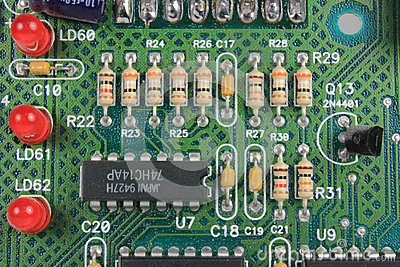
\includegraphics[width=0.5\linewidth]{Figuras/Ch14/associacao.jpg}}
}

\frame{
	\frametitle{Tipos de associações}
	\begin{block}{Pode-se associar os resistores de três maneiras distintas:}
		\begin{itemize}
			\item \textbf{Série}
			\item \textbf{Paralelo}
			\item  Mista
		\end{itemize}
	\end{block}
}

\frame{
	\frametitle{Introdução}
	\begin{block}{Resistor equivalente}
		Para efeito de cálculos, em muitos casos será necessário descobrir como a série de resistores se comporta como um todo. Nestes casos utilizamos o conceito de resistor equivalente.
	\end{block}
	\centerline{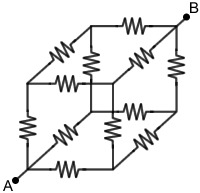
\includegraphics[width=0.4\linewidth]{Figuras/Ch14/req.jpg}}
}

\frame{
	\frametitle{Associação série}
	\centerline{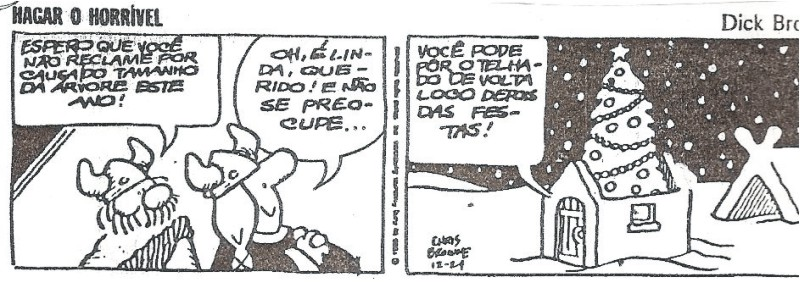
\includegraphics[width=1.1\linewidth]{Figuras/Ch14/natal.jpg}}
}

\frame{
	\frametitle{Associação série}
	\centerline{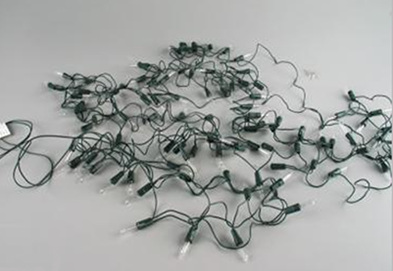
\includegraphics[width=0.9\linewidth]{Figuras/Ch14/natal2.PNG}}
}

\frame{
	\frametitle{Associação série - Corrente}
	\begin{block}{}
		\begin{itemize}
			\item Na associação série existe apenas um caminho para a passagem da \textbf{corrente elétrica}, logo esta é \textbf{mantida} por toda a extensão do circuito.
		\end{itemize}
	\end{block}

	\bigskip

	\centering
	
	\setmyunit{2cm}
	\begin{circuitikz}
		\draw (0,0) to[R,l=$ R_1 $] ++(1,0)
		to[R,l=$ R_2 $,i=$ i $] ++(1,0)
		-- ++(0,-1)
		to[battery1,invert] ++(-2,0)
		-- ++(0,1);
	\end{circuitikz}

%	\centerline{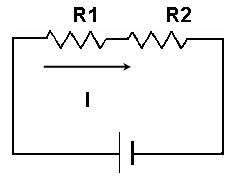
\includegraphics[width=0.4\linewidth]{Figuras/Ch14/seriecorrente.jpg}}
}

\frame{
	\frametitle{Associação série - Tensão}
	\begin{block}{}
		\begin{itemize}
			\item A \textbf{diferença de potencial} entre cada resistor irá \textbf{variar} conforme a resistência deste, para que seja obedecida a 1ª Lei de Ohm.
		\end{itemize}
	\end{block}

	\bigskip

	\centering
	\setmyunit{2cm}
	\begin{circuitikz}
		\foreach \x in {1,2,3,4}{
			\draw ($ (\x,0)+(-1,0) $) to[R,l=$ R_{\x} $,*-*] ++(1,0);
			\draw[<->] ($ (\x,-0.5)+(-1,0) $) -- node[below] {$ U_{\x} $} ++(1,0);
			\draw[dashed] ($ (\x,0)+(-1,0) $) -- ++(0,-0.6);
		}
		
		\draw[<->] (0,-1) -- node[below] {$ U $} ++(4,0);
		\draw[dashed] (0,0) -- ++(0,-1.1);
		\draw[dashed] (4,0) -- ++(0,-1.1);
	\end{circuitikz}
	
%	\centerline{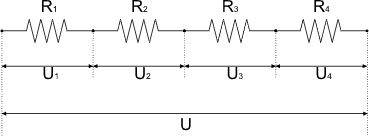
\includegraphics[width=0.8\linewidth]{Figuras/Ch14/serietensao.jpg}}
}

\frame{
	\frametitle{Associação série - Resistência}
	\begin{block}{}
		\begin{itemize}
			\item Em uma associação em série de resistores, o resistor equivalente é igual à \textbf{soma de todos os resistores} que compõem a associação.
			\item Associar resistores em série significa ligá-los em um \textbf{único trajeto}.
		\end{itemize}
	\end{block}

	\bigskip

	\centering
	\setmyunit{2cm}
	\begin{circuitikz}
		\foreach \x in {1,2,3,4}{
			\draw ($ (\x,0)+(-1,0) $) to[R,l=$ R_{\x} $,*-*] ++(1,0);
		}
	\end{circuitikz}
%	\centerline{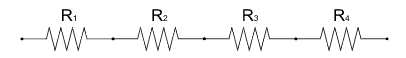
\includegraphics[width=0.9\linewidth]{Figuras/Ch14/serie.PNG}}
}

\frame{
	\frametitle{Associação série}
	\begin{block}{Em resumo...}
		\begin{itemize}
			\item \textbf{Tensão}: se divide
			\item \textbf{Corrente}: se mantém a mesma
			\item \textbf{Resistência equivalente}: soma de cada resistor
		\end{itemize}
	\end{block}
}

\frame{
	\frametitle{Associação série}
	\begin{block}{Exemplo \#01}
		(Fatec – SP) Dois resistores de resistência $R_1 = 5\si{\ohm}$ e $R_2 = 10\si{\ohm}$ são associados em série fazendo parte de um circuito elétrico. A tensão $U_1$ medida nos terminais de $R_1$ é igual a $100$ V. Nessas condições, determine a corrente que passa por $R_2$ e a tensão em seus terminais.
	\end{block}
}

\frame{
	\frametitle{Associação paralelo}
	\centerline{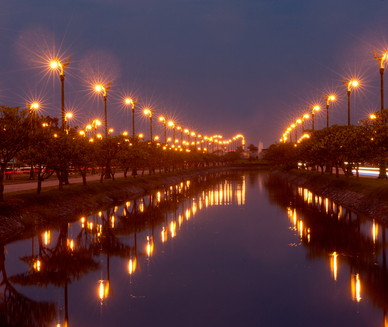
\includegraphics[width=0.7\linewidth]{Figuras/Ch14/paralelo.jpg}}
}

\frame{
	\frametitle{Associação paralelo - Corrente}
	\begin{block}{}
		\begin{itemize}
			\item Ligar um resistor em paralelo significa basicamente \textbf{dividir} a mesma fonte de \textbf{corrente}.
		\end{itemize}
	\end{block}
	
	\medskip
	
	\centering
	\setmyunit{2cm}
	\begin{circuitikz}
		\draw (0,0) to[short,f=$ i $,o-] ++(1,0)
		to[short,i=$ i_2 $,*-] ++(0.5,0)
		to[R,l=$ R_2 $] ++(1,0)
		to[short,i_>=$ i_2 $] ++(0.5,0)
		(1,0) to[short,i=$ i_1 $] ++(0,0.5) -- ++(0.5,0)
		to[R,l=$ R_1 $] ++(1,0) -- ++(0.5,0)
		to[short,i_>=$ i_1 $] ++(0,-0.5)
		(1,0) to[short,i=$ i_3 $] ++(0,-0.5) -- ++(0.5,0)
		to[R,l=$ R_3 $] ++(1,0) -- ++(0.5,0)
		to[short,i_>=$ i_3 $,-*] ++(0,0.5)
		to[short,f=$ i $,-o] ++(1,0);
		
		\draw[dashed] (-0.04,0.1) -- ++(0,-1.2) (4.04,0.1) -- ++(0,-1.2);
		
		\draw[<->] (-0.04,-1) -- node[below] {$ U $} (4.04,-1);
	\end{circuitikz}
	
%	\centerline{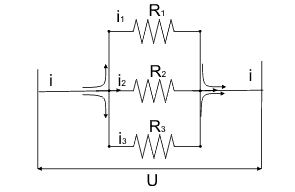
\includegraphics[width=0.4\linewidth]{Figuras/Ch14/paralelocorrente.PNG}}
}

\frame{
	\frametitle{Associação paralelo - Tensão}
	\begin{block}{}
		\begin{itemize}
			\item A \textbf{diferença de potencial} em cada ponto é \textbf{conservada}.
		\end{itemize}
	\end{block}

	\bigskip

	\centering
	\setmyunit{2cm}
	\begin{circuitikz}[european voltages]
		\draw (0,0) to[short,o-*] ++(1,0)
		to[R,v=$ U $] ++(0,-1)
		to[short,*-o] ++(-1,0)
		(1,0) -- ++(1,0)
		to[R,v=$ U $] ++(0,-1) -- ++(-1,0);
	\end{circuitikz}
%	\centerline{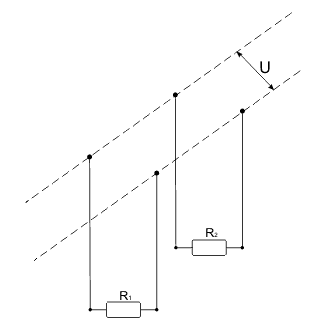
\includegraphics[width=0.55\linewidth]{Figuras/Ch14/paralelotensao.PNG}}
}

\frame{
	\frametitle{Associação paralelo - Resistência}
	\begin{block}{}
		\begin{itemize}
			\item A resistência equivalente de uma associação em paralelo sempre será \textbf{menor} que o resistor de menor resistência da associação.
		\end{itemize}
	
		$$\boxed{\dfrac{1}{R_{eq}} = \dfrac{1}{R_1} + \dfrac{1}{R_2} + \dfrac{1}{R_3} + ... + \dfrac{1}{R_n}}$$
	\end{block}
	
	\bigskip
	
	\centering
	\setmyunit{2cm}
	\begin{circuitikz}
		\draw (0,0) to[short,o-*] ++(1,0)
		to[R,l=$ R_1 $] ++(0,-1)
		to[short,*-o] ++(-1,0)
		(1,0) -- ++(0.5,0)
		to[R,l=$ R_2 $,*-*] ++(0,-1) -- ++(-0.5,0)
		(2.5,0)	to[R,l=$ R_n $] ++(0,-1);
		
		\draw (1.5,0) -- (2,0) (2.2,0) -- (2.5,0) (1.5,-1) -- (2,-1) (2.2,-1) -- (2.5,-1);
		\draw[dotted] (2,0) -- (2.2,0) (2,-1) -- (2.2,-1);
		\draw (2.1,-0.5) node {$ \cdots $};
	\end{circuitikz}
%	\centerline{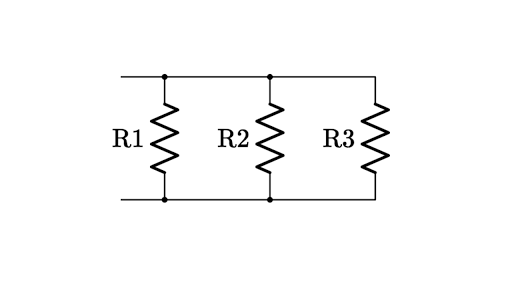
\includegraphics[width=0.6\linewidth]{Figuras/Ch14/paralelo2.png}}
	
}

\frame{
	\frametitle{Associação paralelo - Resistência}
	\begin{block}{Caso especial \#01}
		\begin{itemize}
			\item Quando temos apenas 2 resistores: \\
		\end{itemize}
		$$\boxed{R_{eq} = \dfrac{R_1 \cdot R_2}{R_1 + R_2}}$$
	\end{block}

	\bigskip

	\centering
	\setmyunit{2cm}
	\begin{circuitikz}
		\draw (0,0) to[short,o-*] ++(0.5,0) -- ++(0,0.5)
		to[R,l=$ R_1 $] ++(1,0) -- ++(0,-1)
		to[R,l=$ R_2 $] ++(-1,0) -- ++(0,0.5)
		(1.5,0) to[short,*-o] ++(0.5,0);
	\end{circuitikz}
%	\centerline{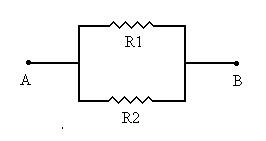
\includegraphics[width=0.6\linewidth]{Figuras/Ch14/resistores2.jpg}}
}

\frame{
	\frametitle{Associação paralelo - Resistência}
	\begin{block}{Caso especial \#02}
		\begin{itemize}
			\item Quando temos $n$ resistores de valores iguais ($R$): \\
		\end{itemize}
		$$\boxed{R_{eq} = \dfrac{R}{n}}$$
	\end{block}

	\bigskip
	
	\centering
	\setmyunit{2cm}
	\begin{circuitikz}
		\draw (0,0) to[short,o-*] ++(1,0)
		to[R,l=$ R_1{=}R $] ++(0,-1)
		to[short,*-o] ++(-1,0)
		(1,0) -- ++(1,0)
		to[R,l=$ R_2{=}R $,*-*] ++(0,-1) -- ++(-1,0)
		(3.5,0)	to[R,l=$ R_n{=}R $] ++(0,-1);
		
		\draw (2,0) -- (2.9,0) (3.1,0) -- (3.5,0) (2,-1) -- (2.9,-1) (3.1,-1) -- (3.5,-1);
		\draw[dotted] (2.9,0) -- (3.1,0) (2.9,-1) -- (3.1,-1);
		\draw (3,-0.5) node {$ \cdots $};
	\end{circuitikz}

%	\centerline{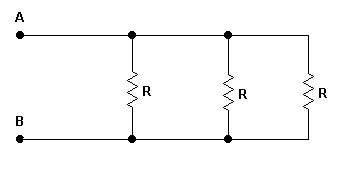
\includegraphics[width=0.6\linewidth]{Figuras/Ch14/paraleloigual.png}}
}

\frame{
	\frametitle{Associação paralelo}
	\begin{block}{Em resumo...}
		\begin{itemize}
			\item \textbf{Tensão}: se mantém a mesma
			\item \textbf{Corrente}: se divide
			\item \textbf{Resistência equivalente}: sempre menor que a resistência de menor valor que o circuito apresenta.
		\end{itemize}
	\end{block}
}

\frame{
	\frametitle{Associação paralelo}
	\begin{block}{}
		Sobre um circuito que contém apenas uma associação de resistores em paralelo, é INCORRETO afirmar que:

		(a) A corrente total do circuito é igual à soma das correntes individuais de cada resistor; \\

		(b) A ddp em cada resistor é igual à tensão elétrica fornecida pela fonte;

		(c) A resistência equivalente é sempre menor do que a resistência de menor valor que o circuito contém;

		(d) A corrente elétrica é igual em todos os resistores;

		(e) Se um resistor queima, a corrente elétrica que circula nos demais componentes do circuito não se altera.
	\end{block}
}

\frame{
	\frametitle{Associação série x paralelo}
	\begin{block}{Importante}
		\begin{itemize}
			\item Quando um dos resistores da associação em paralelo queima, a corrente elétrica que circula nos demais componentes do circuito não é alterada.
			\item Os circuitos elétricos residenciais e de iluminação pública são todos em paralelo
		\end{itemize}
	\end{block}
	\centerline{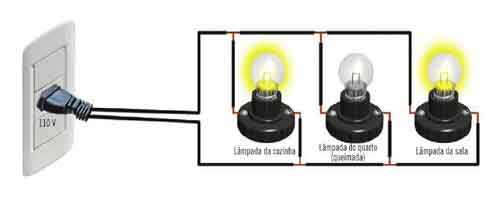
\includegraphics[width=0.6\linewidth]{Figuras/Ch14/lampadaqueimada.jpg}}
}

% https://exercicios.brasilescola.uol.com.br/exercicios-fisica/exercicios-sobre-associacao-resistores---serie.htm#questao-1


\section*{Exercícios}

\frame{
	\frametitle{Exercícios}
	\begin{block}{}
		01. (PUC-RJ) Quando as resistências $R_1$ e $R_2$ são colocadas em série, elas possuem uma resistência equivalente de $\SI{6}{\ohm}$. Quando $R_1$ e $R_2$ são colocadas em paralelo, a resistência equivalente cai para $\SI[]{4/3}{\ohm}$. Quais são os valores das resistências $R_1$ e $R_2$?

		\vspace{0,5cm}

		02. Considere a associação de resistores em paralelo da figura a seguir, e determine: (a) a resistência equivalente no circuito; (b) a ddp em cada resistor; (c) a corrente elétrica em cada resistor; (d) a corrente elétrica total.
	\end{block}

	\centering
	\setmyunit{2cm}
	\begin{circuitikz}
		\draw (0,0) to[battery1=120<\volt>,f<_=$ i $] ++(0,-1.5) -- ++(3,0)
		(0,0) -- ++(1,0) to[R=10<\ohm>,i=$ i_1 $,*-*] ++(0,-1.5)
		(1,0) -- ++(1,0) to[R=15<\ohm>,i=$ i_2 $,*-*] ++(0,-1.5)
		(2,0 )-- ++(1,0) to[R=12<\ohm>,i=$ i_3 $,*-*] ++(0,-1.5);
	\end{circuitikz}
%	\centerline{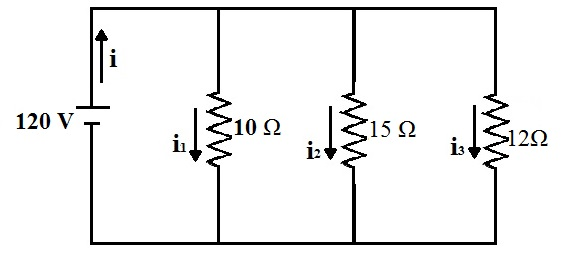
\includegraphics[width=0.6\linewidth]{Figuras/Ch14/paraleloexemplo.jpg}}
}

\section*{Referências}

\frame{
	\frametitle{Referências e Exercícios Complementares}
	\begin{itemize}
		\item Física, Ciência e Tecnologia – Vol 3. PENTEADO, Paulo César M; TORRES, Carlos Magno A. Ed. Moderna (2006)
	\end{itemize}
	%\centering{\alert{Página 36 - \textbf{1.6.1 até 1.6.5, 1.6.17 até 1.6.19}}} \\
	\centering{\alert{Lista de exercícios 14}}
}